% ---------------------------------------------------------------------------
% Splatt3R-SLAM -- CVPR-format manuscript
%
% Build:  latexmk -pdf main.tex        (or: pdflatex -> bibtex -> pdflatex x2)
%
% Fonts: this document deliberately uses ONLY the Type 1 fonts bundled with
% every TeX Live / MiKTeX distribution (URW Nimbus Roman via the `times`
% package required by cvpr.sty, plus Nimbus Sans and Computer Modern math).
% No system font is referenced, so the PDF builds byte-comparably on Linux
% and Windows with pdflatex. Do NOT switch to XeLaTeX/fontspec: that would
% pull in OS-installed fonts and break cross-platform reproducibility.
% ---------------------------------------------------------------------------
\documentclass[10pt,twocolumn,letterpaper]{article}

%%%%%%%%% PAPER TYPE  (pick one)
% \usepackage{cvpr}              % review mode: line numbers + anonymous
\usepackage[final]{cvpr}         % camera-ready / preprint
% \usepackage[pagenumbers]{cvpr} % preprint with page numbers

\usepackage{graphicx}
\usepackage{amsmath}
\usepackage{amssymb}
\usepackage{booktabs}
\usepackage{multirow}
\usepackage{xcolor}
\usepackage{cuted}

\definecolor{cvprblue}{rgb}{0.21,0.49,0.74}
\usepackage[pagebackref,breaklinks,colorlinks,citecolor=cvprblue]{hyperref}

\def\paperID{****}
\def\confName{CVPR}
\def\confYear{2026}

% Convenience macros used throughout the tables.
\newcommand{\best}[1]{\textbf{#1}}
\newcommand{\dB}{\,dB}
\newcommand{\up}{$\uparrow$}
\newcommand{\dn}{$\downarrow$}

\begin{document}

\title{Splatt3R-SLAM: Feed-Forward Gaussian Splatting for Real-Time Dense SLAM,\\
and an Honest Account of What It Costs}

\author{Zelong Li\\
{\tt\small loong.li2@student.uva.nl}\\
{\tt\small +31\,6\,3023\,2998}
}

\maketitle
\begin{strip}
  \centering
  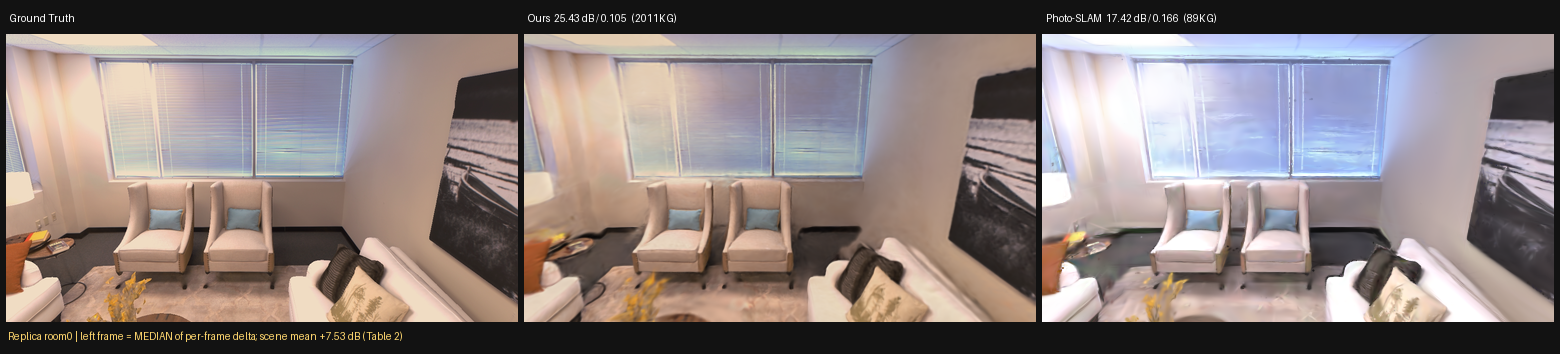
\includegraphics[width=\linewidth]{fig/cmp_replica_room0_f0.png}
  \captionof{figure}{\textbf{Novel-view rendering on Replica room0, all three
  panels scored under one protocol} (\cref{sec:protocol}): a held-out frame
  that is a keyframe of neither system, rendered from the ground-truth pose
  Sim(3)-aligned into each map's own frame, through one renderer and one
  metric implementation. The frame shown is the \emph{median} of the per-frame
  $\Delta$PSNR distribution, not a hand-picked one --- an arbitrarily chosen
  frame on this scene can reverse the ordering
  (\cref{sec:exp:replica}). Our map reaches this quality with
  $2.0$M Gaussians against Photo-SLAM's $89$K; \cref{sec:lim:compact} shows
  that the size is load-bearing rather than redundant.}
  \label{fig:teaser}
\end{strip}


\begin{abstract}
Feed-forward two-view Gaussian predictors remove the per-scene optimisation
that dense Gaussian-splatting SLAM normally requires, but a predictor trained
on curated image pairs is not automatically a good \emph{map} builder: a SLAM
system fuses hundreds of keyframes over the same surfaces, a regime the
pairwise training objective never observes. We integrate Splatt3R into
MASt3R-SLAM and study what actually has to change for the fused map, rather
than the individual prediction, to improve.

We report three results. First, adaptation must be confined to the Gaussian
head: fine-tuning the frozen encoder with LoRA collapses reconstruction by
$49\%$, while head-only training of the same budget improves deployed map
quality on five dataset families. Second, a training-free lever --- fading
Gaussian opacity at map-assembly time in proportion to pointmap confidence ---
improves the online map in $10$ of $12$ cells with zero harmful cells, and we
show why a training-time penalty cannot substitute for it. Third, we identify
what opacity does in this architecture: it is a brightness-trim dial against
the black-background rasteriser, not a confidence gate. A pre-registered
opposite-sign prediction (opacity versus input luminance, negative for heads
trained under synthetic darkening and positive for real-sensor heads) holds on
$5/5$ families, and unifies the first two results.

We then build all four comparison systems from source and evaluate every
system through one protocol. Two findings follow that we believe matter beyond
this system. (i) Published GS-SLAM rendering numbers and ours differ by
roughly one protocol, not by quality: running Photo-SLAM ourselves yields
$22.2$\dB{} on Replica office0 where the literature reports ${\sim}30.9$\dB{}
for the same system, an offset independently reproduced as an $8.8$\dB{} gap
between rendering a map from its own estimated poses versus ground-truth
poses. (ii) Our own headline advantage shrinks under scrutiny: on all eight
Replica scenes we lead Photo-SLAM by $+3.44$\dB{} PSNR but win LPIPS on only
$5/8$, and a three-scene subset would have overstated the margin by
$1.85$\dB{}. Most importantly, our maps carry $25$--$100\times$ more
primitives and $8$--$16\times$ more GPU memory, and pruning them to a
baseline's budget costs $8.7$--$10.3$\dB{} --- the map size is load-bearing,
not padding. We report the compactness deficit as a measured architectural
limitation rather than a footnote.
\end{abstract}

\section{Introduction}
\label{sec:intro}

Dense visual SLAM has converged on 3D Gaussian splatting~\cite{kerbl20233dgs}
as its map representation, because Gaussians render photorealistically in real
time where neural fields~\cite{mildenhall2020nerf} do not. The dominant
designs --- MonoGS~\cite{matsuki2024monogs},
Photo-SLAM~\cite{huang2024photoslam}, SplaTAM~\cite{keetha2024splatam} ---
obtain their Gaussians by \emph{per-scene optimisation}: primitives are
initialised, then densified and refined by gradient descent against the
incoming frames.

A different route has become available. Feed-forward reconstruction networks
predict geometry directly from images without optimisation:
DUSt3R~\cite{wang2024dust3r} regresses pointmaps from an image pair,
MASt3R~\cite{leroy2024mast3r} adds matching, and
Splatt3R~\cite{smart2024splatt3r} extends MASt3R with a head that emits a full
Gaussian per pixel --- position, covariance, colour and opacity --- in a single
forward pass. MASt3R-SLAM~\cite{murai2025mast3rslam} shows that the MASt3R
prior supports real-time dense tracking. The combination is therefore
attractive: a SLAM system whose map appears at the speed of a forward pass.

The difficulty is a mismatch of regimes. Splatt3R is trained on
\emph{curated image pairs}, and its loss sees exactly two views at a time. A
SLAM system does something categorically different: it fuses hundreds of
keyframes onto the same physical surfaces, so every surface is covered many
times over, by predictions made from different viewpoints, at different
exposures, with different confidences. Nothing in pairwise training observes
this crowding. Our starting observation is that a checkpoint which is
excellent per pair can nonetheless produce a fused map that is hazy and
over-solid --- and that fixing this is not a matter of training longer.

This paper asks what actually has to change, and reports the answer as three
results.

\paragraph{Where adaptation is admissible.}
The obvious move --- adapt the backbone to the target domain --- fails
decisively. Encoder LoRA~\cite{hu2022lora} degrades reconstruction by $49\%$
with a $1821\times$ scale explosion, and decoder-only LoRA improves for one
epoch then collapses. The reason is structural: Splatt3R's Gaussian head was
trained against \emph{frozen} encoder features, and perturbing those features
feeds the head inputs it has never seen. Training only the Gaussian head, with
the encoder bit-frozen, improves deployed map quality across five dataset
families. Because the encoder is untouched, tracking is unchanged by
construction --- a property we verify externally rather than assume.

\paragraph{A training-free lever, and why training cannot replace it.}
Fading each Gaussian's opacity at the moment it is injected into the map, in
proportion to how little the pointmap vouches for it, improves the online map
in $10$ of $12$ cells across four families, six heads and eight scenes, with
two ties and \emph{no} harmful cell. This is not a heuristic that a better
loss would subsume: crowding is a map-level property that only exists after
many keyframes accumulate, and a pair-training objective never sees a map. We
support this with a dose--response experiment at two thinning depths.

\paragraph{What opacity is.}
Both preceding results turn out to be the same result. We show that opacity in
this architecture is a \emph{brightness-trim dial} against the
black-background rasteriser, not the confidence or hedging channel it is
usually assumed to be: because the colour term is anchored to the (possibly
degraded) input pixel and is sigmoid-bounded, opacity is the only channel with
headroom to brighten. The decisive evidence is a pre-registered opposite-sign
prediction --- heads trained under synthetic darkening should correlate opacity
\emph{negatively} with input luminance, real-sensor heads \emph{positively} ---
which holds on all five families. Under this account the base checkpoint's
collapsed opacity means it \emph{cannot} trim; injection-time thinning supplies
the trim externally; and heads that deploy well are the ones that learned it.

\paragraph{An honest comparison, and what it cost us.}
We built MASt3R-SLAM, MonoGS, Photo-SLAM and VGGT-SLAM~\cite{maggio2025vggtslam}
from source and evaluated every system --- ours included --- through a single
protocol, on held-out views that are keyframes of no system. Two findings
emerged that we did not set out to make.

First, \emph{published GS-SLAM rendering numbers are not comparable to ours},
and the gap is quantifiable. Running Photo-SLAM ourselves on Replica office0
gives $22.2$\dB{} where third-party tables report ${\sim}30.9$\dB{} for the
same system. We independently reproduce an $8.8$\dB{} gap on MonoGS between
rendering its own map from its own estimated poses versus ground-truth poses.
Two systems, two methods, the same ${\sim}8.7$\dB{}: the literature and this
paper differ by one protocol's worth of evaluation choices.

Second, several of our own claims weakened when pushed. A three-scene Replica
subset suggested a $+5.29$\dB{} advantage; completing all eight scenes reduced
it to $+3.44$\dB{} and revealed that we win LPIPS on only $5/8$. On TUM at
matched compute we \emph{tie} MonoGS on PSNR and \emph{lose} on LPIPS. And our
maps carry $25$--$100\times$ more Gaussians at $8$--$16\times$ the peak memory;
pruned to a baseline's budget our quality falls $8.7$--$10.3$\dB{}
\emph{below} it, so the size is constitutive rather than redundant. We report
these as measured results, with the curve, rather than as caveats.

Our contributions are: (i) a head-only adaptation recipe for feed-forward
Gaussian SLAM, with the negative encoder-adaptation result that motivates it;
(ii) an injection-time thinning lever with a dose--response argument for why
training cannot substitute for it; (iii) a falsifiable mechanism for opacity,
confirmed by a pre-registered opposite-sign prediction on $5/5$ families;
(iv) a single-protocol comparison against four locally-built systems, with a
quantified protocol offset that we believe affects how this literature should
be read; and (v) a measured account of the efficiency deficit our
representation carries.

\section{Related Work}
\label{sec:related}

\paragraph{Feed-forward 3D reconstruction.}
DUSt3R~\cite{wang2024dust3r} recasts two-view stereo as direct regression of
aligned pointmaps, removing explicit correspondence search;
MASt3R~\cite{leroy2024mast3r} adds a matching head and metric scale, and
VGGT~\cite{wang2025vggt} generalises the formulation to many views.
Splatt3R~\cite{smart2024splatt3r} builds on MASt3R by freezing the encoder and
decoder and training only a Gaussian head that emits, per pixel, a covariance,
spherical-harmonic colour and opacity (\cref{eq:mu}--\cref{eq:splatt3rloss}).
That freezing decision is not incidental for us: it is the reason the head is
brittle to any change in its input features, which we quantify in
\cref{sec:method:head}. A second consequence matters equally: because
\cref{eq:splatt3rloss} is masked, purely photometric and strictly pairwise, the
training objective is blind to every property that only emerges when hundreds
of keyframes are fused --- which is precisely the regime a SLAM map occupies.

\paragraph{Gaussian-splatting SLAM.}
MonoGS~\cite{matsuki2024monogs} optimises Gaussians and camera poses jointly by
gradient descent from monocular video. Photo-SLAM~\cite{huang2024photoslam}
couples ORB-SLAM3~\cite{campos2021orbslam3} tracking with a
Gaussian mapping thread. SplaTAM~\cite{keetha2024splatam} and
Gaussian-SLAM~\cite{yugay2023gaussianslam} take related routes with RGB-D
input. All of these obtain map primitives by per-scene optimisation, and their
map quality is therefore a function of the optimisation budget they are given
--- a dependency we make explicit when comparing
(\cref{sec:experiments}). Our system differs in that primitives arrive
\emph{predicted}: the optimiser refines an initialisation that is already
approximately correct, rather than creating structure.

\paragraph{Feed-forward priors inside SLAM.}
DROID-SLAM~\cite{teed2021droidslam} established learned dense optimisation for
tracking. MASt3R-SLAM~\cite{murai2025mast3rslam} uses the MASt3R prior for
real-time dense tracking and pointmap fusion, and is the system we build on;
we inherit its tracking front-end unmodified, which is why our trajectory
accuracy matches it and why we are explicit that trajectory accuracy is
\emph{not} a contribution of this work.
VGGT-SLAM~\cite{maggio2025vggtslam} aligns VGGT submaps on the $SL(4)$
manifold; it produces poses and a point cloud but no renderable map, so in our
comparison it serves as a tracking control rather than a rendering baseline.

\paragraph{Parameter-efficient adaptation.}
LoRA~\cite{hu2022lora} is the default tool for adapting a large frozen
backbone. Our experience is a cautionary counterexample: for a pipeline whose
downstream head was \emph{trained against frozen features}, perturbing the
backbone is not a mild intervention, and we measure a $49\%$ collapse. The
useful adaptation surface in such architectures is the head itself.

\paragraph{Evaluation practice.}
Rendering quality in this literature is reported as PSNR/LPIPS~\cite{zhang2018lpips}
and trajectory accuracy as ATE after Sim(3) alignment~\cite{umeyama1991},
typically via evo~\cite{grupp2017evo}. The details underneath those names vary
substantially between papers --- whether scoring views are training or held-out,
whether rendering uses estimated or ground-truth poses, resolution,
undistortion, and post-sequence optimisation budget. \Cref{sec:protocol} shows
that these choices are worth roughly $8.7$\dB{} on unchanged systems, which is
larger than most reported inter-method differences.

\section{Preliminaries}
\label{sec:prelim}

\subsection{Feed-forward pointmaps and Gaussians}
DUSt3R~\cite{wang2024dust3r} maps an uncalibrated image pair
$I^i, I^j \in \mathbb{R}^{H\times W\times 3}$ to pointmaps
$X^i_i, X^j_i \in \mathbb{R}^{H\times W\times 3}$ with confidences
$C^i_i, C^j_i$, where $X^i_j$ denotes the pointmap of image $i$ expressed in
the frame of camera $j$. MASt3R~\cite{leroy2024mast3r} adds a matching head
producing features $D^i_i, D^j_i \in \mathbb{R}^{H\times W\times d}$. We write
$F_M(I^i, I^j)$ for one forward pass.

Splatt3R~\cite{smart2024splatt3r} adds a third head, in parallel to the
pointmap and matching heads and using the same DPT decoder, which emits for
every pixel a rotation quaternion $q\in\mathbb{R}^4$, a scale
$s\in\mathbb{R}^3$, spherical-harmonic coefficients
$S\in\mathbb{R}^{3\times d}$, an opacity $\alpha\in\mathbb{R}$ and a mean
offset $\Delta\in\mathbb{R}^3$, so that the Gaussian centre is
\begin{equation}
\mu \;=\; x + \Delta, \qquad x \in X^i_i .
\label{eq:mu}
\end{equation}
Quaternions are normalised, scales and offsets pass through an exponential and
opacities through a sigmoid. Critically for this paper, \emph{only the Gaussian
head is trained}: the encoder and decoder remain those of the pre-trained
MASt3R model, and all Gaussian parameters are predicted in the first image's
camera frame, avoiding any ground-truth transformation at inference.

The covariance follows the standard 3DGS~\cite{kerbl20233dgs} parameterisation
\begin{equation}
\Sigma \;=\; R(q)\,\mathrm{diag}(s)^2\,R(q)^\top ,
\label{eq:cov}
\end{equation}
and a view with world-to-camera $W$ and projective Jacobian $J$ renders with
the projected covariance $\Sigma' = J W \Sigma W^\top J^\top$, compositing
front-to-back:
\begin{equation}
c \;=\; \sum_{k} c_k\,\alpha_k \prod_{l<k}\bigl(1-\alpha_l\bigr).
\label{eq:alphacomp}
\end{equation}
\Cref{eq:alphacomp} is the reason opacity behaves as it does in our analysis
(\cref{sec:method:mech}): with a black background, the residual transmittance
$\prod_l (1-\alpha_l)$ contributes zero radiance, so lowering $\alpha$ darkens
a region and raising it brightens it.

Splatt3R is supervised only by novel-view renderings, under a mask $M$ of
pixels visible in at least one context view:
\begin{equation}
\mathcal{L} = \lambda_{\text{MSE}}\,\mathcal{L}_{\text{MSE}}(M\!\odot\!\hat{I}, M\!\odot\!I)
            + \lambda_{\text{LP}}\,\mathcal{L}_{\text{LPIPS}}(M\!\odot\!\hat{I}, M\!\odot\!I),
\label{eq:splatt3rloss}
\end{equation}
with $\lambda_{\text{LP}}{=}0.25$ in the released configuration. Two properties
of \cref{eq:splatt3rloss} drive our method. It is \emph{purely photometric} ---
depth enters only through the mask $M$ and through pair selection, never
through a gradient on geometry --- and it is \emph{pairwise}: the loss never
observes more than two context views, hence never observes a fused map.

In the released implementation the DC colour is anchored to the source image:
the head predicts a residual which is added to the spherical-harmonic encoding
of the input RGB value,
\begin{equation}
S_{\mathrm{DC}}(u)=S_{\mathrm{res}}(u)+\operatorname{RGB2SH}(I^i(u)).
\label{eq:colorresidual}
\end{equation}
Consequently, revisits can inherit exposure, white-balance, shadow, and
view-dependent differences from their source frames. Exposure normalisation
removes only the global component of this source-frame photometric gauge; it
does not enforce equality of $S_{\mathrm{DC}}$ for the same world surface.

\subsection{SLAM back-end}
We inherit MASt3R-SLAM's~\cite{murai2025mast3rslam} front- and back-end
unchanged. Poses are $\mathrm{Sim}(3)$ to absorb the scale inconsistency of
network predictions,
\begin{equation}
T=\begin{bmatrix} sR & t\\ 0 & 1\end{bmatrix},\qquad
T \leftarrow \tau \oplus T \triangleq \mathrm{Exp}(\tau)\circ T ,
\label{eq:sim3}
\end{equation}
with $\tau\in\mathfrak{sim}(3)$. Under a generic central-camera assumption a
pointmap induces its own camera model through the ray map
$\psi(X^i_i)$ (unit-norm normalisation), and tracking minimises a ray error
rather than a 3D point error, because
$\lVert\psi_1-\psi_2\rVert^2 = 2(1-\cos\theta)$ is bounded and therefore
robust to the depth errors that pointmap prediction frequently exhibits. The
canonical keyframe pointmap is maintained by a confidence-weighted running
average,
\begin{equation}
\tilde X^k_k \leftarrow
\frac{\tilde C^k_k \tilde X^k_k + C^f_k\, T_{kf} X^f_k}{\tilde C^k_k + C^f_k},
\qquad
\tilde C^k_k \leftarrow \tilde C^k_k + C^f_k .
\label{eq:fusion}
\end{equation}
Loop closures enter a $\mathrm{Sim}(3)$ pose graph solved by Gauss--Newton.
We modify none of this; the consequence is that our tracking is identical to
MASt3R-SLAM by construction, which \cref{sec:exp:ate} verifies externally.

\section{Method}
\label{sec:method}

\subsection{System}
We replace the pointmap prediction with Splatt3R, so each keyframe pair yields
a per-pixel Gaussian in one forward pass. Keyframe Gaussians are stored in
their anchor keyframe's local frame and composed into the world through that
keyframe's \emph{current} pose,
\begin{equation}
\mu^{W} = A_k\,\mu^{k} + b_k, \qquad
\Sigma^{W} = A_k\,\Sigma^{k}\,A_k^{\top},
\label{eq:anchor}
\end{equation}
where $[A_k\,|\,b_k]$ is the $\mathrm{Sim}(3)$ matrix of keyframe $k$. Because
the composition reads the pose at render time, a loop closure that updates
$T_{WC_k}$ moves the map with it at no cost and without re-baking --- the
property our refinement design depends on
(\cref{sec:method:refiner}).

The implementation stores means, scales, rotations, SH coefficients, opacity,
confidence, and validity in a shared keyframe buffer. Tracker updates may
rewrite pointmap state without clearing the Gaussian record unless a new
Gaussian prediction is present. This invariant prevents a geometric update
from silently erasing an already renderable keyframe. Filtering and the
global Gaussian limit are applied before rasterisation; the limit is therefore
a rendering budget implemented through spatial stride, rather than FIFO
deletion of individual keyframes.

\subsection{Where adaptation is admissible}
\label{sec:method:head}

Splatt3R trains its head against \emph{frozen} encoder features, making the
head a function of one specific feature distribution. We measured what happens
when that distribution moves:

\begin{itemize}\itemsep2pt
\item \textbf{Encoder LoRA}~\cite{hu2022lora} ($r{=}8$, $\alpha{=}16$ on
      \texttt{qkv}/\texttt{proj}/\texttt{fc1}/\texttt{fc2}, $46.6$M trainable):
      $-49\%$ reconstruction quality against the released checkpoint, with
      predicted scales exploding by $1821\times$. The failure is immediate,
      not a late-training instability.
\item \textbf{Decoder-only LoRA}: $+0.37$\dB{} at epoch~1, then collapse to
      $-1.61$\dB{} by epoch~5 with a $12\times$ climb in the $99$th-percentile
      scale.
\item \textbf{Head-only} (encoder and decoder bit-frozen, only
      \texttt{gaussian\_dpt} trainable): improves, and is what we keep.
\end{itemize}

The interpretation is structural rather than a matter of hyper-parameters. The
scale head is exponentially parameterised, $s = \exp(\hat{s})$, so it is
unconstrained above; feeding the head out-of-distribution features perturbs
$\hat{s}$ in a regime where the photometric loss of \cref{eq:splatt3rloss} is
nearly flat --- a large, nearly transparent Gaussian and a small opaque one
render almost identically at the supervision views. Geometry is therefore free
to diverge while the loss barely moves, which is exactly the observed
signature (quality collapse with scale explosion). Head-only training keeps
$46.6$M parameters frozen and trains the $158$M-parameter head with the
upstream objective and Adam~\cite{kingma2015adam}, per dataset family.

\subsection{Injection-time thinning}
\label{sec:method:thin}

A SLAM map covers each surface with predictions from many keyframes. Under
\cref{eq:alphacomp} with a black background, a surface covered by many
over-solid Gaussians composites to haze rather than to a sharper surface. We
therefore fade opacity at the moment a Gaussian enters the map, in proportion
to how little the pointmap confidence vouches for it.

Confidences are not calibrated across keyframes, so we rank-normalise
\emph{within} each keyframe. For a keyframe with $N$ Gaussians and confidence
values $\{c_n\}$, let $r_n$ be the rank of $c_n$ and
$\hat{c}_n = r_n/(N-1) \in [0,1]$. The injected opacity is
\begin{equation}
\alpha'_n \;=\; \alpha_n \cdot
\mathrm{clip}\Bigl(1 - 2\lambda\,(1-\hat{c}_n),\; 0.1,\; 1\Bigr),
\label{eq:thin}
\end{equation}
with dose $\lambda{=}0.45$ shipped. The lower clip at $0.1$ is deliberate: it
keeps \cref{eq:thin} a \emph{thinning} prior rather than a deletion prior, so
that even the least-confident Gaussian retains gradient and the refiner can
recover it if the photometric evidence supports it.

\paragraph{Why a training-time penalty cannot substitute.}
An opacity penalty added to \cref{eq:splatt3rloss} would be a different
intervention, because crowding \emph{does not exist} at training time: it is a
property of the assembled map, which forms only after SLAM accumulates
keyframes over a surface, and \cref{eq:splatt3rloss} never sees more than two
context views. Consistent with this, we measured that the refiner
un-saturates opacity on its own even with an untrained head (median
$1.0\rightarrow0.26$), identifying thinning as an \emph{acceleration along a
path the optimiser already walks} --- which also explains its bounded
downside, since a prior the optimiser would have reached anyway cannot do much
harm. A dose--response check at two thinning depths (opacity knees $0.9$ and
$0.6$) gave $-21.0\%$ and $-15.8\%$ LPIPS; neither collapsed toward zero, as a
training-substitutable effect would require.

\subsection{Online map refinement}
\label{sec:method:refiner}

Prediction gives a good initialisation, not a converged map. We add a third
process that photometrically refines the assembled map \emph{while SLAM runs}.

\paragraph{Parameterisation.}
Gaussians are optimised in their anchor keyframe's local frame in
pre-activation form --- $\log s$, unnormalised $q$, $\mathrm{logit}\,\alpha$,
and the SH DC term --- so that scales stay positive and opacity stays in
$(0,1)$ without constraints, and composed to the world by
\cref{eq:anchor} at every step. Per-group Adam rates follow the 3DGS
reference, with the positional rate scaled by scene extent:
$\eta_\mu = 1.6\!\times\!10^{-4}\!\cdot\!\mathrm{extent}$,
$\eta_{f_{dc}} = 2.5\!\times\!10^{-3}$, $\eta_\alpha = 5\!\times\!10^{-2}$,
$\eta_s = 5\!\times\!10^{-3}$, $\eta_q = 1\!\times\!10^{-3}$.

\paragraph{Objective.}
Supervision views are tracked frames, so the refiner optimises
\begin{equation}
\mathcal{L}_{\text{ref}} = (1-\lambda_{D})\,\lVert \hat{I}-I \rVert_1
                          + \lambda_{D}\,\bigl(1-\mathrm{SSIM}(\hat{I},I)\bigr),
\qquad \lambda_{D}=0.2 ,
\label{eq:refloss}
\end{equation}
i.e.\ the 3DGS objective rather than \cref{eq:splatt3rloss}: LPIPS is a
reporting metric here, not a training signal, so that our evaluation metric is
not also our loss.

\paragraph{Anchor-carried supervision.}
Each supervision frame is stored as an image together with
$(\text{anchor index}, T_{\text{anchor},f})$ rather than a world pose. Its
world pose is recomposed through the anchor's \emph{current} pose at sample
time, so supervision follows loop closures exactly as the map does under
\cref{eq:anchor}. Frames are held in CPU shared memory, which is what allows
the refiner to run on a second GPU without pinning both processes to one card.
If frame $f$ is anchored to keyframe $k$, the stored relative transform gives
\begin{equation}
T_{WC_f}=T_{WC_k}T_{C_kC_f}.
\label{eq:supervisionpose}
\end{equation}
The refiner consequently never becomes a second pose-graph writer: a loop
closure changes the anchor pose once, and both map placement and supervision
views follow that correction.

\paragraph{Sampling.}
Supervision is drawn from a reservoir of $200$ frames spanning the whole
sequence plus a ring of the $64$ most recent, with a recent fraction of $0.3$.
We measured uniform-over-history to dominate a recency-weighted schedule
(held-out early/late split: $14.40/14.09/14.72$ uniform versus
$14.06/13.79/14.35$ recent-only), because causal arrival already biases the
pool toward recent views.

\paragraph{Scheduling.}
Sharing one GPU, the refiner holds a duty cycle $d$ by sleeping
$\mathrm{EMA}[\Delta t]\,(1-d)/d$ after each step, so optimisation steps are
dropped but never frames. Refiner load on the \emph{same} card doubles tracker
latency ($101\!\rightarrow\!206$\,ms p50); on a second card it is noise
($103$\,ms), which is the configuration we deploy. After the sequence ends an
optional polish phase continues with the final poses.

\paragraph{Frozen centres.}
We hold $\mu$ fixed during refinement. The centres come from the network's
pointmap, and photometric gradients degrade them: because the loss of
\cref{eq:refloss} is evaluated at the supervision views themselves, moving a
centre can reduce training error while worsening the geometry seen from new
viewpoints. This was measured optimal at both online ($\sim$300-step) and
offline (3000-step) budgets.

The refiner publishes a versioned CPU snapshot rather than mutable GPU state.
The visualiser uploads only complete versions and retains the previous valid
version on a read/write collision. If the display buffer is smaller than the
refined map, publication subsamples after the full map has been saved. This
separates bounded display memory from the evaluation artifact and prevents a
large-map publication failure from discarding a valid refinement result.

\subsection{What opacity is}
\label{sec:method:mech}

The two preceding levers are, we argue, one phenomenon. Consider what the
architecture permits. The DC colour is anchored to the input pixel plus a
small learned residual and is sigmoid-bounded, so it cannot brighten a region
much past what its input pixel suggests. Under \cref{eq:alphacomp} with a black
background, $\alpha$ can: lowering it darkens toward black, raising it
brightens by admitting less background. Opacity is therefore the only channel
with headroom to \emph{lift} content --- a brightness-trim dial, not the
confidence or hedging gate it is usually taken to be.

This makes a falsifiable, sign-specific prediction. Let $\ell$ be input
luminance and $\rho$ the Spearman correlation between $\alpha$ and $\ell$ over
predicted Gaussians. A head trained with independently darkened inputs
(synthetic vignetting and white-balance jitter, where the target view's
darkening cannot be inferred from the input) must learn to lift what the input
darkened, so $\rho<0$. A head trained on real sensor data with no synthetic
darkening should instead place solid Gaussians on bright, reliably
reconstructable content, so $\rho>0$. We registered both signs before
measuring; \cref{sec:exp:mech} reports the result.

\section{Evaluation Protocol}
\label{sec:protocol}

Every number in this paper was produced by us on one machine
($2{\times}$RTX~A6000). All four comparison systems were built from source
locally; \emph{no number is copied from a paper}. This section states the
protocol before the results, because we will show that the protocol is worth
more than most of the differences it is used to measure.

\subsection{One protocol for every system}
Rendering quality is scored identically for all systems:
\begin{itemize}\itemsep2pt
\item \textbf{Scoring views:} $100$ held-out frames per scene, selected to be
      keyframes of \emph{no} participating system, so every scored view is
      genuinely unseen by all of them.
\item \textbf{Rendering pose:} ground-truth pose, Sim(3)-aligned~\cite{umeyama1991}
      into each map's own (arbitrary, monocular) frame.
\item \textbf{Renderer and metrics:} one code path, one PSNR and one
      LPIPS~\cite{zhang2018lpips} implementation, one exposure-normalisation
      setting, for every system.
\item \textbf{Sensor parity:} monocular against monocular.
\end{itemize}
Trajectory accuracy is ATE~RMSE via \texttt{evo\_ape tum -as}~\cite{grupp2017evo}.

\paragraph{Datasets.} Rendering is evaluated on all eight
Replica~\cite{straub2019replica} scenes and on TUM
RGB-D~\cite{sturm2012tum} \texttt{freiburg1}; trajectory accuracy on all nine
TUM \texttt{freiburg1} sequences. Head-only adaptation
(\cref{sec:exp:head}) additionally uses EuRoC~\cite{burri2016euroc},
ETH3D~\cite{schops2017eth3d} and 7-Scenes~\cite{shotton2013scenecoord},
giving five dataset families in total.

\paragraph{Alignment.}
Each monocular map lives in its own arbitrary $\mathrm{Sim}(3)$ frame, so
ground-truth poses must be transported into it. We fit
$(s,R,t)$ by Umeyama's closed-form solution~\cite{umeyama1991} on the
estimated/ground-truth camera-centre pairs and invert it,
\begin{equation}
R_{\text{map}} = R^{\top} R_{\text{gt}},\qquad
t_{\text{map}} = R^{\top}\bigl(t_{\text{gt}}-t\bigr)/s ,
\label{eq:align}
\end{equation}
noting that the $1/s$ belongs to the translation only --- folding it into the
rotation block yields a non-orthonormal matrix that silently corrupts every
rendered viewpoint. Systems that log both estimated and ground-truth keyframe
poses (MonoGS) are aligned from those pairs directly; the rest from their
trajectory files.

\subsection{A mandatory self-consistency check}
\label{sec:protocol:selfcheck}
Before any cross-system number is reported we require that \emph{a map must
render well from the poses it was built at}. This is not a formality. Our first
MonoGS adapter assumed its logged trajectory was world-to-camera when it is
camera-to-world; the inverted convention scored MonoGS at $4.36$\dB{} against
$18.71$\dB{} for the correct one, and would have produced a large, flattering,
publishable-looking margin. We adopted the rule that a result which favours us
receives one more verification step than one that does not; it changed our
conclusion three separate times.

\subsection{The protocol offset}
\label{sec:protocol:offset}

Two independent measurements quantify how much the protocol is worth on
\emph{unchanged} systems.

\noindent\textbf{(i) Same system, our protocol versus the literature.}
Photo-SLAM built from its own source scores $22.23$\dB{} on Replica office0
under our protocol; third-party comparison tables report ${\sim}30.9$\dB{} for
Photo-SLAM on monocular Replica. Offset: $\mathbf{8.7}$\dB{}.

\noindent\textbf{(ii) Same map, two pose sources.}
Taking MonoGS's own output map and changing only the rendering pose:
$18.71$\dB{} from its own estimated poses, $9.87$\dB{} from ground-truth poses.
Offset: $\mathbf{8.8}$\dB{}.

Two different systems, two different methods, essentially the same figure. We
conclude that GS-SLAM rendering numbers in the literature and ours differ by
approximately one protocol's worth of evaluation choices --- scoring on
training versus held-out views, estimated versus ground-truth poses,
resolution, undistortion, and post-sequence optimisation budget --- rather than
by quality. Concretely, our Replica $23.0$\dB{} mean should \emph{not} be read
as trailing a published $30.9$\dB{}: measured identically, we are ahead of the
system that published it.

\paragraph{What the offset is made of.}
We can attribute part of it directly. Scoring the \emph{same} map from
estimated versus ground-truth poses is worth $8.8$\dB{} on MonoGS and
$2.6$\dB{} on Photo-SLAM, the difference between the two reflecting how much
each system's map has co-adapted to its own pose error. Beyond pose source,
the protocols we found differ in: whether keyframes are excluded from scoring
(MonoGS excludes its own; Photo-SLAM's self-reported PSNR is computed
\emph{on} its keyframes), resolution ($640\!\times\!480$ undistorted versus our
$512\!\times\!384$), masking (PSNR over $I_{gt}>0$ pixels only), and
post-sequence optimisation budget ($26{,}000$ iterations for MonoGS versus our
$300$\,s polish). We do not claim to have decomposed the offset exactly; we
claim that it is large, reproducible, and larger than most reported
inter-method differences.

\paragraph{Reporting rule.} We therefore tabulate only numbers we produced
under one protocol. Published numbers are cited in text where relevant but are
never placed in a comparison table beside our own. We recommend this practice
generally for this literature.

\subsection{Systems compared}
\Cref{tab:systems} lists what each system can contribute. Two of the four
produce no renderable map and therefore appear only in the trajectory table;
MonoGS ships RGB-D-only Replica configurations, so including it there against
our monocular system would give it a depth-input advantage and we omit it
rather than report an unfair win.

\begin{table}[t]
\centering
\small
\setlength{\tabcolsep}{4pt}
\begin{tabular}{@{}llcl@{}}
\toprule
System & Type & Rend. & Role here \\
\midrule
Ours & mono 3DGS & \checkmark & --- \\
Photo-SLAM & mono 3DGS & \checkmark & rendering \\
MonoGS & mono 3DGS & \checkmark & rendering (TUM) \\
MASt3R-SLAM & mono dense & --- & tracking control \\
VGGT-SLAM & pose+cloud & --- & tracking control \\
\bottomrule
\end{tabular}
\caption{Systems compared: Photo-SLAM~\cite{huang2024photoslam},
MonoGS~\cite{matsuki2024monogs}, MASt3R-SLAM~\cite{murai2025mast3rslam},
VGGT-SLAM~\cite{maggio2025vggtslam}. The latter two produce no renderable map
--- we verified by source inspection that the VGGT-SLAM repository contains no
rasteriser or photometric metric --- so they appear only in the trajectory
table. MASt3R-SLAM is the system we inherit tracking from, making it a control
rather than an opponent.}
\label{tab:systems}
\end{table}

\section{Experiments}
\label{sec:experiments}

\subsection{Head-only adaptation}
\label{sec:exp:head}
Head-only training was run per dataset family and evaluated on the deployed
map, not on validation pairs. Deployed LPIPS improves on four of five
families: ETH3D $-29.1\%$, EuRoC $-20.8\%$, TUM $-7.9\%$ to $-25.9\%$ over
four sequences, Replica positive, and 7-Scenes the weak family
($+0.14\%$ to $-4.9\%$). The result is seed-robust: two heads $\times$ two
seeds, checked at both validation and deployment level, gave relative deltas
under $5\%$ with inconsistent signs --- ordinary noise rather than fragility.

\paragraph{Four falsified attributions.}
We attempted to explain why some families gain far more than others, and
failed. \Cref{tab:falsified} lists the candidates: each was pre-registered
with the cell that would refute it, and each was refuted by direct
measurement rather than by argument. We report this as a negative result. The
gains are real --- they exceed a measured $0.17\%$ LPIPS noise floor --- but we
decline to adopt the most plausible surviving story in the absence of an
out-of-sample test.

\begin{table}[t]
\centering\small
\setlength{\tabcolsep}{3pt}
\begin{tabular}{@{}p{0.30\linewidth}p{0.62\linewidth}@{}}
\toprule
Candidate & Why it fails \\
\midrule
Scale-frame consistency &
Mechanically inert: \cref{eq:splatt3rloss} is purely photometric, means are
\texttt{detach()}ed, and the metric-scale flag's only consumer is disabled.
Depth touches training solely via the mask. \\
Supervision coverage &
Measured per family: EuRoC has the \emph{lowest} coverage ($39.5\%$) and the
second-largest gain; ETH3D matches TUM's coverage ($61.9$ vs $60.0\%$) with
$3\times$ the gain. \\
Opacity un-saturation &
Explains four families in rank order but 7-Scenes measures $0.479$ ---
comparable to EuRoC's $0.38$ --- with a null gain. A measured counterexample,
not a pending cell. \\
Base-checkpoint headroom &
$\rho=0.145$ over $11$ sequences. ETH3D \texttt{sofa\_1} has the lowest
deficit of any sequence and the second-largest gain. \\
\bottomrule
\end{tabular}
\caption{Four pre-registered mechanisms for the cross-family variation, each
killed by measurement. The variation is real and remains unattributed.}
\label{tab:falsified}
\end{table}

\begin{figure*}[t]
  \centering
  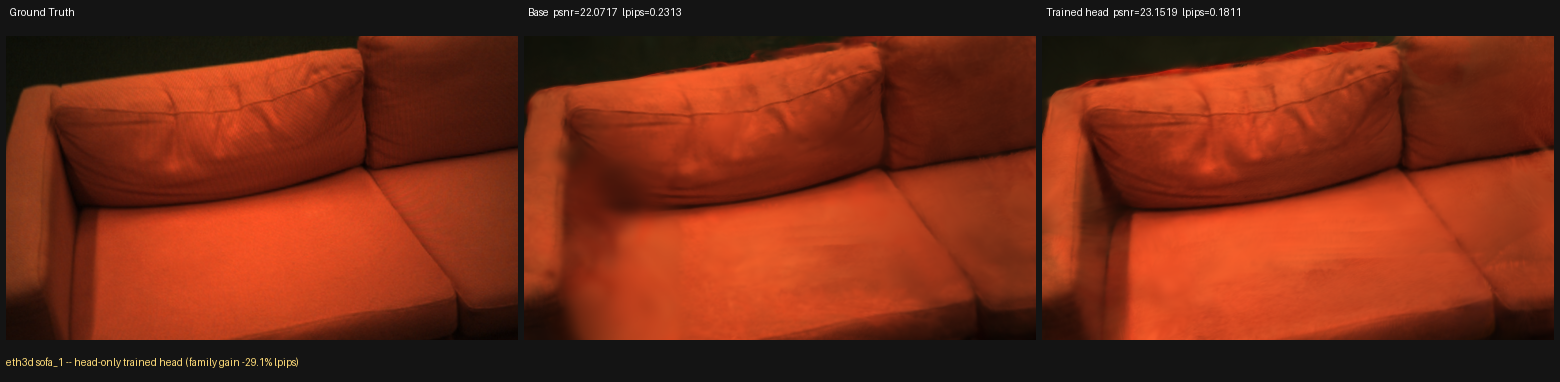
\includegraphics[width=0.92\linewidth]{fig/eth3d_sofa1_f1.png}\\[2pt]
  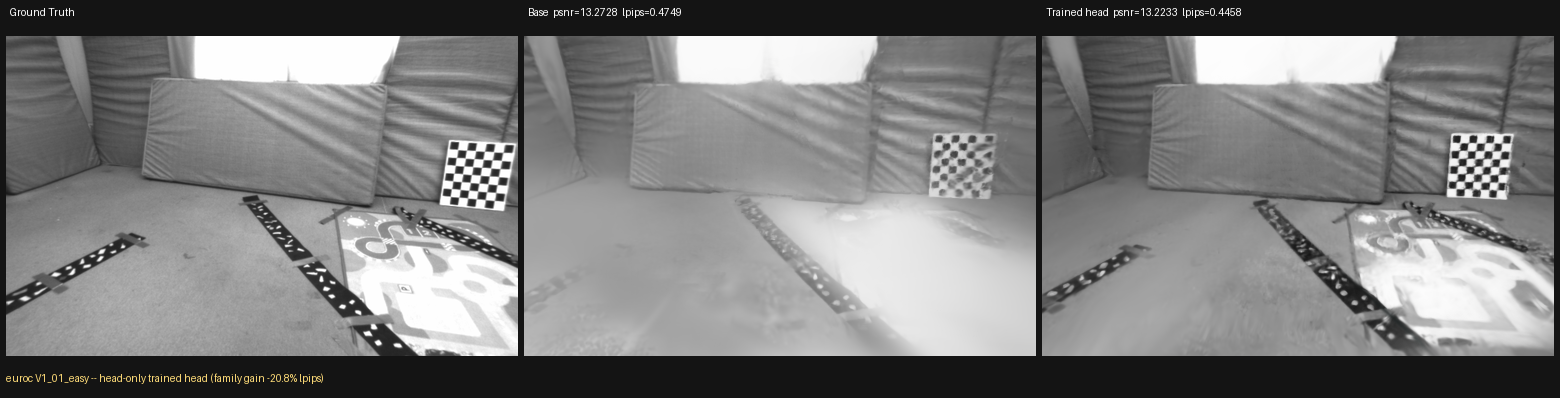
\includegraphics[width=0.92\linewidth]{fig/euroc_v101_f0.png}\\[2pt]
  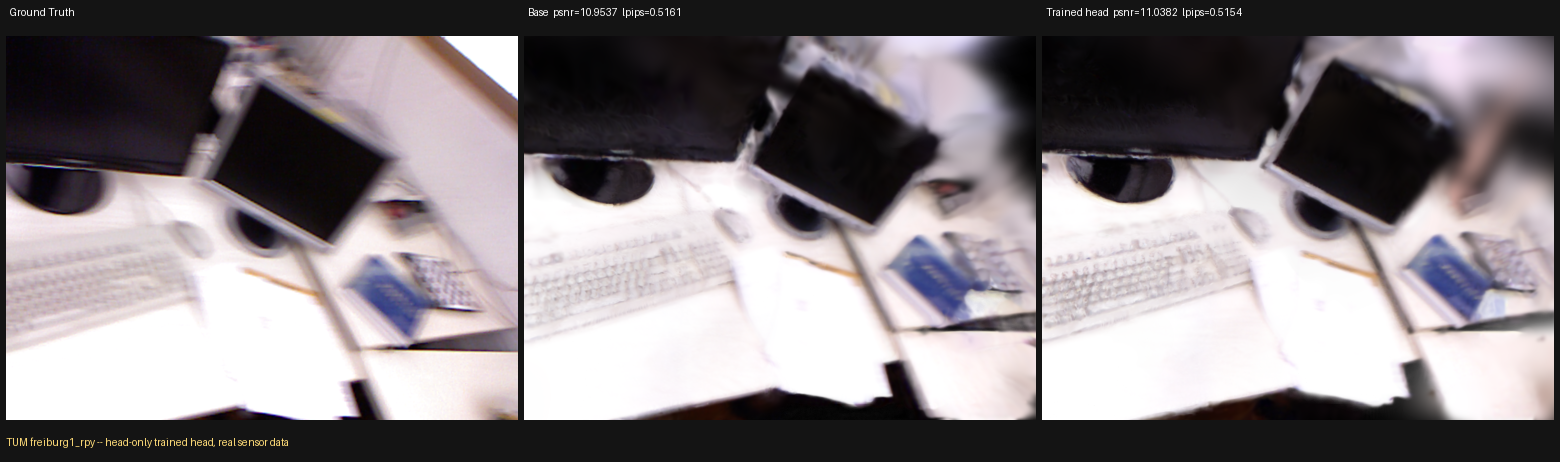
\includegraphics[width=0.92\linewidth]{fig/tum_rpy_f0.png}\\[2pt]
  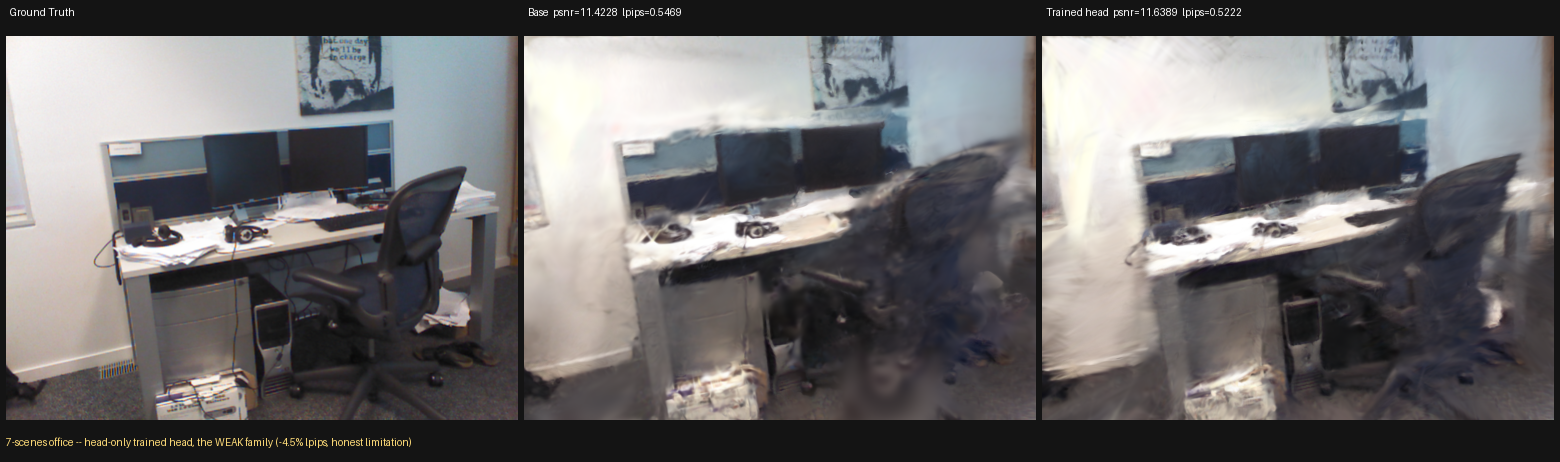
\includegraphics[width=0.92\linewidth]{fig/7scenes_office_f0.png}
  \caption{\textbf{Head-only adaptation, per family} (ground truth $|$ released
  checkpoint $|$ head-only fine-tuned), on held-out non-keyframe views. Rows:
  ETH3D \texttt{sofa\_1}, EuRoC \texttt{V1\_01}, TUM \texttt{fr1\_rpy},
  7-Scenes \texttt{office}. The first three are families where the recipe
  clearly helps; the last is the weak family
  ($+0.14\%$ to $-4.9\%$ LPIPS), included so the failure mode is visible rather
  than only tabulated. Because the encoder is bit-frozen, the difference
  between the second and third panel of each row is attributable to the
  Gaussian head alone.}
  \label{fig:headonly}
\end{figure*}

\subsection{Injection-time thinning}
\label{sec:exp:thin}
Across $12$ online cells spanning four families, six heads and eight scenes:
$10$ clear benefits, $2$ ties, $0$ harmful cells, worst cell $+0.16\%$ LPIPS.
The confidence-weighted allocation of \cref{eq:thin} is shipped as the default,
though we note honestly that confidence-weighted versus uniform allocation is
statistically a coin flip at this sample size (median $-0.06\%$, CI containing
zero); we ship it because it is never much worse and it is the configuration
all deployment comparisons were run with.

\paragraph{Dose--response.}
If the effect were something a training-time penalty could supply, thinning
should lose its benefit once the head already produces well-separated
opacities. We measured two thinning depths on heads whose opacity distributions
differ, obtaining $-21.0\%$ and $-15.8\%$ LPIPS: neither collapsed toward
zero. Together with the observation that the refiner un-saturates opacity
unaided (median $1.0\rightarrow0.26$), this supports the reading of
\cref{eq:thin} as an acceleration of a trajectory the optimiser already
follows, rather than as information the network was missing.

\subsection{The opacity mechanism}
\label{sec:exp:mech}
\Cref{tab:lum} reports the pre-registered test. Heads trained under synthetic
darkening correlate opacity \emph{negatively} with input luminance; heads
trained on real sensor data correlate \emph{positively}. All five families
land on the predicted sign, with magnitudes clustering tightly.

\begin{table}[t]
\centering\small
\begin{tabular}{@{}llr@{}}
\toprule
Head & Training data & $\rho(\alpha,\text{luminance})$ \\
\midrule
photospatial & Replica + synthetic darkening & $-0.316$ \\
mixed        & Replica + synthetic darkening & $-0.279$ \\
TUM          & real sensor                   & $+0.303$ \\
ETH3D        & real sensor                   & $+0.392$ \\
EuRoC        & real sensor                   & $+0.304$ \\
\bottomrule
\end{tabular}
\caption{Pre-registered opposite-sign prediction, confirmed on $5/5$ families.
Both signs were registered before any number was computed.}
\label{tab:lum}
\end{table}

\subsection{Rendering: Replica, all eight scenes}
\label{sec:exp:replica}
\Cref{tab:replica} is the load-bearing rendering comparison: monocular against
monocular, on the benchmark this literature actually uses for rendering.

\begin{table}[t]
\centering\small
\setlength{\tabcolsep}{3.5pt}
\begin{tabular}{@{}lcccc@{}}
\toprule
\multirow{2}{*}{Scene} & \multicolumn{2}{c}{Ours} & \multicolumn{2}{c}{Photo-SLAM} \\
\cmidrule(lr){2-3}\cmidrule(lr){4-5}
 & PSNR\up & LPIPS\dn & PSNR\up & LPIPS\dn \\
\midrule
office0 & \best{26.30} & \best{0.104} & 22.23 & 0.209 \\
office1 & \best{22.08} & \best{0.115} & 17.80 & 0.185 \\
office2 & \best{20.97} & 0.151 & 20.24 & \best{0.129} \\
office3 & \best{20.18} & \best{0.144} & 19.36 & 0.155 \\
office4 & \best{23.65} & 0.156 & 16.46 & \best{0.125} \\
room0   & \best{25.44} & \best{0.110} & 17.92 & 0.152 \\
room1   & \best{21.91} & \best{0.140} & 21.88 & 0.175 \\
room2   & \best{23.62} & 0.160 & 20.75 & \best{0.116} \\
\midrule
Mean    & \best{23.02} & \best{0.135} & 19.58 & 0.156 \\
\bottomrule
\end{tabular}
\caption{Replica, monocular, one protocol. We lead PSNR on $8/8$ but LPIPS on
only $5/8$. A three-scene subset (office0, office1, room0) would have reported
$+5.29$\dB{}; all eight give $+3.44$\dB{}, and three scenes are effectively
ties ($+0.03$, $+0.73$, $+0.81$).}
\label{tab:replica}
\end{table}

\begin{figure*}[t]
  \centering
  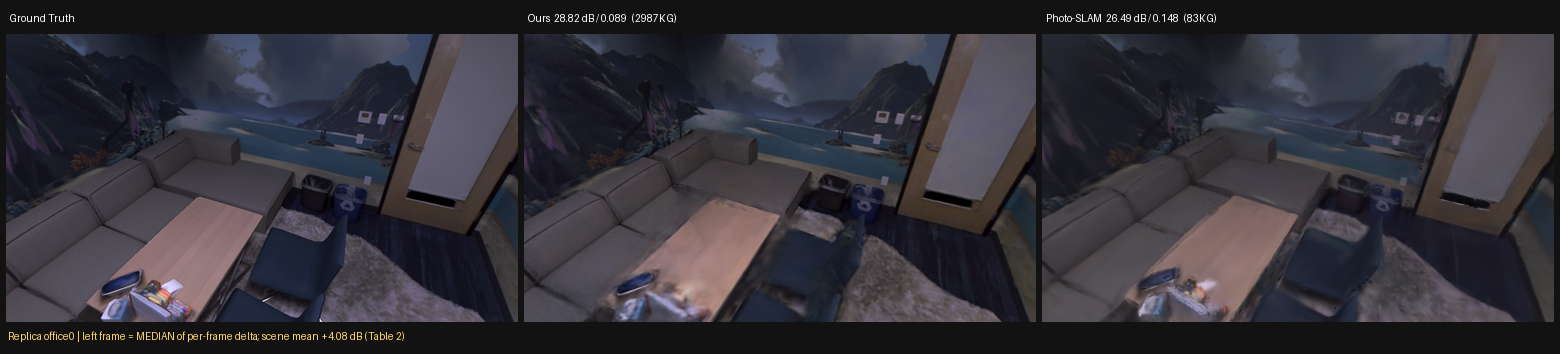
\includegraphics[width=0.92\linewidth]{fig/cmp_replica_office0_f1.png}
  \caption{\textbf{Replica office0, one protocol.} A second baseline comparison
  under the identical protocol used for \cref{fig:teaser}, on a scene where our
  margin is closer to the Replica mean ($+4.08$\dB{} versus the $+3.44$\dB{}
  eight-scene mean) rather than at the top of the range.}
  \label{fig:office0}
\end{figure*}

\paragraph{Means hide the distribution.}
Scoring $24$ probe frames per scene individually, the per-frame $\Delta$PSNR
median is $+8.01$ on room0 and $+3.62$ on office0, but $\mathbf{-1.84}$ on
office2 --- a scene whose \emph{mean} says we lead by $+0.73$\dB{}. Our nominal
win there comes from a minority of frames, not from being typically better.
Even on room0, Photo-SLAM wins some frames ($\min\Delta = -4.77$). Qualitative
figures in this paper are therefore selected at the median of the per-frame
delta, not by eye.

\subsection{Rendering: TUM, and the budget question}
\label{sec:exp:tum}
\Cref{tab:tum} reports TUM \texttt{fr1\_desk}, the only TUM sequence where all
three rendering systems track successfully. At \emph{matched wall clock} ---
our $300$\,s polish against MonoGS's $339$\,s refinement --- PSNR ties and
MonoGS wins LPIPS. Only with $3.5\times$ their budget do we lead both. The
honest statement is that MonoGS has better perceptual quality at equal compute
and we can buy past it with more, not that our deficit was a budget artefact.

\begin{table}[t]
\centering\small
\setlength{\tabcolsep}{4pt}
\begin{tabular}{@{}lccrr@{}}
\toprule
System & PSNR\up & LPIPS\dn & Gauss. & Budget \\
\midrule
Ours ($300$\,s)   & 13.95 & 0.411 & 2.40M & $\sim$1.4k st. \\
MonoGS ($339$\,s) & 13.87 & \best{0.398} & \best{23K} & 26k it. \\
Photo-SLAM        & 10.73 & 0.558 & 36K & to shutdown \\
\midrule
Ours ($1200$\,s)  & \best{14.61} & \best{0.379} & 2.40M & $\sim$4.4k st. \\
\bottomrule
\end{tabular}
\caption{TUM \texttt{fr1\_desk}. This comparison cannot be extended to further
TUM sequences: MonoGS's monocular tracking diverges on them
(\cref{tab:ate}), and scoring rendering against a diverged map would measure
tracking failure rather than rendering quality.}
\label{tab:tum}
\end{table}

\subsection{Trajectory accuracy}
\label{sec:exp:ate}
\Cref{tab:ate} completes the trajectory picture. The finding is
\emph{robustness}, not precision: Photo-SLAM and MonoGS each diverge on
several sequences ($0.30$--$0.84$\,m, i.e.\ failure rather than error), which
is what dominates their means, while on sequences they do track Photo-SLAM is
frequently the most accurate. We stress that our parity with MASt3R-SLAM
(4--4--1, noise) is \emph{expected and not a contribution}: the tracking
front-end is inherited unchanged, which \cref{tab:ate} verifies externally
rather than by assertion.

\begin{table}[t]
\centering\small
\setlength{\tabcolsep}{3pt}
\begin{tabular}{@{}lrrrrr@{}}
\toprule
Seq. & Ours & MASt3R & VGGT & Photo & MonoGS \\
\midrule
360   & 0.042 & 0.048 & 0.050 & \best{0.035} & 0.177 \\
desk  & 0.017 & 0.016 & 0.025 & \best{0.015} & 0.036 \\
desk2 & \best{0.028} & 0.024 & 0.029 & 0.438 & 0.844 \\
floor & 0.027 & 0.025 & 0.099 & \best{0.013} & 0.539 \\
plant & \best{0.015} & 0.020 & 0.025 & 0.046 & 0.071 \\
room  & \best{0.059} & 0.061 & 0.064 & 0.510 & 0.791 \\
rpy   & 0.022 & 0.023 & 0.026 & 0.057 & \best{0.041} \\
teddy & 0.048 & 0.045 & \best{0.036} & 0.305 & 0.123 \\
xyz   & 0.009 & 0.009 & 0.014 & \best{0.010} & 0.017 \\
\midrule
Mean  & \best{0.030} & 0.030 & 0.041 & 0.161 & 0.293 \\
\bottomrule
\end{tabular}
\caption{ATE RMSE (m), TUM freiburg1, all nine sequences and all five systems.
Photo-SLAM is non-deterministic (ORB-SLAM3 is multi-threaded): \texttt{desk}
gave $0.0174$ and $0.0149$ on two runs, so its single-run figures carry
run-to-run variance.}
\label{tab:ate}
\end{table}

\subsection{Front-end geometry is not the lever}
\label{sec:exp:frontend}
\Cref{tab:ate} raises an obvious design question, and we answer it by
measurement rather than argument. The per-keyframe scale jitter behind the
visible seams in our maps is a two-view artefact: each cluster's scale is
decided by one independent forward, and neighbouring clusters are decided by
different ones. Would our contributions therefore be better carried by a joint
many-view front-end such as VGGT-SLAM~\cite{maggio2025vggtslam}? We ran that
question in four stages. It is a negative result, and it has a mechanism.

\paragraph{Joint context removes the jitter; a better backbone does not.}
We measure adjacent-view depth-scale disagreement against RGB-D depth in a
gauge-free form --- per window, the spread of the scale each view implies,
normalised so that no global gauge enters. \Cref{tab:scale} is the resulting
$2\times2$. The \emph{same} VGGT~\cite{wang2025vggt} weights on the
\emph{same} pairs are $2.0\times$ \emph{worse} than the incumbent two-view
backbone when run pairwise, and $6.4\times$ better when sixteen views are
coupled in one forward. Changing the architecture makes it worse; changing the
context makes it better. The gain is attributable to multi-view context, not
to a stronger prior --- and our deployment regime is the causal two-view one,
which is precisely VGGT's weakest mode. A drop-in backbone swap would buy the
$10.82\%$ row, not the $1.68\%$ one.

\paragraph{Averaging cannot substitute for coupling.}
The cheap version of the same idea needs no new backbone: at keyframe
creation, predict the new view against $m$ well-overlapping partners,
scale-align the $m$ depth maps and average. Measured over
$m\in\{1,2,4,8\}$ this saturates at $5.16\%\rightarrow3.06\%$ --- a factor of
two above what coupling reaches, at $m$ forwards per keyframe. Independent
draws cancel; a gauge does not.

\paragraph{The referee is right, and the picture gets worse.}
We then used one joint sixteen-view forward over all of a map's keyframes as
an external scale referee, taking the per-cluster scalar corrections it
implies --- normalised to median one, so the map's global scale is untouched
--- and applying them to the baked map. Absolute per-keyframe scale error
against the sensor improves $6.35\times$ ($6.48\%\rightarrow1.02\%$ on
\texttt{fr1\_desk}; $2.2$--$2.3\times$ on \texttt{360} and \texttt{room}),
and held-out PSNR \emph{falls} from $12.35$ to $11.50$\dB{} with LPIPS rising
$0.507\rightarrow0.523$. A $300$\,s polish does not recover it
($13.81\rightarrow13.08$). The obvious escape --- that the referee is
incompetent on SLAM keyframes, which are selected to be as dissimilar as
possible, unlike the consecutive views it was validated on --- was audited by
scoring map and referee against the sensor on exactly those keyframes: the
referee is $2.2$--$6.4\times$ the more accurate of the two. The referee is
right and the rendering still degrades.

\paragraph{The same conflict inside the refiner.}
Supplying the corrections as a \emph{prior} rather than an edit, with keyframe
translations freed so the photometric term is able to disagree, is monotone in
the prior weight and monotone the wrong way: PSNR $13.74\rightarrow13.38$ and
LPIPS $0.449\rightarrow0.456$ as the weight goes $0.05\rightarrow0.5$, and
even at the largest weight the fitted scale spread is $2.6\%$ against the
referee's $8.0\%$. The photometric term is still winning the argument, and
forcing it further is what the previous paragraph already measured as harmful.

\paragraph{What this establishes.}
In a trajectory-anchored map, rendered quality is not governed by absolute
geometric accuracy. SLAM fits each keyframe's pose to that keyframe's own
biased pointmap, so much of the per-cluster scale error is \emph{common-mode}
with the pose. The photometric evaluation is structurally blind to common-mode
depth error at these baselines --- $4.5\%$ of depth is $0.66$\,px at
\texttt{fr1\_desk}'s $0.057$\,m median keyframe baseline --- but it is not
blind to two overlapping clusters disagreeing about where a surface is, and
correcting a cluster alone converts an absorbed error into exactly that
differential displacement. The two objectives do not even agree in rank: the
photometric fit asks for a $0.8\%$ per-keyframe correction where the sensor
says the map is $6.5\%$ wrong, with Spearman $+0.06$ between them. Every
post-hoc per-cluster geometric correction is therefore closed, and the jitter
can only be removed where poses and per-keyframe scales are solved
\emph{together} --- in the back-end, which is a different system rather than a
component swap. This is why our front-end is inherited unchanged, and it is
also why a joint front-end is not a shortcut to our open problems: VGGT-SLAM
already costs $9{,}436$\,MiB (\cref{sec:exp:cost}) while producing no
renderable map at all.

\begin{table}[t]
\centering\small
\setlength{\tabcolsep}{5pt}
\begin{tabular}{@{}llrr@{}}
\toprule
Predictor & Context & Views & Disagreement \dn \\
\midrule
Splatt3R (deployed) & pairwise & 2 & $5.35\%$ \\
VGGT~\cite{wang2025vggt} & pairwise & 2 & $10.82\%$ \\
VGGT~\cite{wang2025vggt} & joint & 16 & \best{$1.68\%$} \\
\midrule
\multicolumn{4}{@{}l}{\emph{disjoint-window replication}} \\
Splatt3R & pairwise & 2 & $4.92\%$ \\
VGGT & joint & \phantom{0}8 & \best{$1.53\%$} \\
\bottomrule
\end{tabular}
\caption{Adjacent-view depth-scale disagreement, gauge-free, TUM freiburg1,
pooled over seven sequences ($84$ windows above the rule, $33$ disjoint
windows below it). Windows in the primary arm overlap by $80$--$97\%$, so the
result is replicated on eight-view windows tiled by exactly one span; the
replication is $7/7$ sequences, paired Wilcoxon $p=8.6\times10^{-8}$. VGGT's
$1.68\%$ sits at or below the RGB-D sensor's own view-dependent bias floor, so
it is a lower bound on how far coupling goes.}
\label{tab:scale}
\end{table}

\subsection{Refinement ablations}
\label{sec:exp:refiner}
\Cref{tab:refiner} isolates the components of \cref{sec:method:refiner}. The
refiner's own contribution, measured with the base checkpoint on both arms so
that only the refiner toggles, is large and consistent across families:
$+8.69$\dB{} on ETH3D, $+4.62$\dB{} on Replica, $+3.52$\dB{} on TUM and
$+1.00$\dB{} on EuRoC. This is not a marginal add-on next to head-only
training --- on ETH3D it exceeds it --- and the two levers stack rather than
compete.

\begin{table}[t]
\centering\small
\setlength{\tabcolsep}{4pt}
\begin{tabular}{@{}lrl@{}}
\toprule
Ablation & $\Delta$PSNR & Note \\
\midrule
Refiner on, ETH3D   & $+8.69$ & 300\,s polish \\
Refiner on, Replica & $+4.62$ & \\
Refiner on, TUM     & $+3.52$ & \\
Refiner on, EuRoC   & $+1.00$ & \\
\midrule
Causal replay, 120 it. & $+1.21$ & strict real time \\
Second GPU, unthrottled & $+2.15$ & latency $+1\%$ \\
\midrule
Uniform vs.\ recency & $+0.34$ & held-out mean \\
Voxel dedup, 10\,mm & $-0.53$ & $-27.6\%$ map size \\
\bottomrule
\end{tabular}
\caption{Refinement ablations. ATE is unchanged in every row
($0.016975$ vs.\ a $0.0170$ baseline in the deterministic configuration): the
map is strictly downstream of tracking, and the pre-registered failure
condition ``ATE moves at all'' never fired. Freezing the Gaussian centres was
separately measured optimal at both the online ($\sim$300-step) and offline
(3000-step) budgets. The dedup row is included as a negative: it is a map-size
control that costs quality when it fires without a recovery budget, not a
quality feature.}
\label{tab:refiner}
\end{table}

\subsection{Online delivery across dataset families}
\label{sec:exp:online}
The offline ablations above use a controlled polish budget. We therefore also
ran the actual deployed path: a per-family head, causal SLAM, GUI enabled, and
the refiner on the second GPU. \Cref{tab:online} reports the paired map
quality; the refiner never receives or writes a pose correction.

\begin{table}[t]
\centering\small
\setlength{\tabcolsep}{2.7pt}
\begin{tabular}{@{}llrrrr@{}}
\toprule
Family & Sequence & Bake P & Refine P & $\Delta$P & $\Delta$L \\
\midrule
TUM & desk & 12.42 & 13.75 & +1.33 & $-7.5\%$ \\
TUM & room & 11.15 & 11.45 & +0.30 & $+11.1\%$ \\
TUM & 360 & 12.00 & 12.14 & +0.14 & $+20.6\%$ \\
7-Scenes & chess & 13.44 & 13.79 & +0.35 & $-4.8\%$ \\
7-Scenes & office & 11.64 & 11.74 & +0.10 & $-1.6\%$ \\
7-Scenes & pumpkin & 14.15 & 14.91 & +0.77 & $-4.1\%$ \\
EuRoC & MH\_01 & 10.17 & 11.67 & +1.50 & $-4.1\%$ \\
EuRoC & V1\_01 & 12.06 & 12.69 & +0.63 & $-13.0\%$ \\
ETH3D & plant\_1 & 20.42 & 22.22 & +1.80 & $-7.4\%$ \\
\bottomrule
\end{tabular}
\caption{Actual GUI-on, dual-GPU online delivery. P is PSNR in dB and L is
LPIPS; $\Delta L$ is relative, so negative is better. Seven of nine cells
improve LPIPS. TUM room and 360 gain a little PSNR but lose perceptual quality
under the in-sequence budget, exposing supervision starvation on their large
maps rather than a universal refiner improvement. ETH3D \texttt{cables\_1} is
omitted because its $0.5$-m scene and $0.1165$-m ATE make held-out rendering
alignment-dominated. The reported online values are from the pre-polish
delivery pass; the longer polish diagnostic is separated below.}
\label{tab:online}
\end{table}

The deployment cost is measurable rather than merely architectural. Across
the nine online runs, the second-GPU refiner costs approximately $7$--$10\%$
frame time with the GUI open. The head-only arm uses $19.8$--$39.6$~GB on
GPU0; enabling refinement adds $1$--$1.5$~GB on GPU0 and $2.8$--$14.0$~GB on
GPU1, with the largest observed combination $41.1$~GB plus $14.0$~GB on the
two cards. These measurements define the practical operating envelope: the
refiner is deployable, but memory remains proportional to the assembled map.

\paragraph{Budget, not a simple position prior.}
The online TUM room/360 degradation initially suggested a position-learning
rate failure. That explanation came from an offline proxy and did not survive
the causal loop. The deployed sequences supplied only $104/114/190$ refiner
steps for desk/360/room maps, whereas a post-sequence polish producing
$1581/3821/1856$ steps improved PSNR by $+1.97/+2.30/+2.22$~dB and LPIPS by
$-22.0/-8.3/-15.9\%$, respectively. We therefore reverted the offline
position-freezing and band-limit defaults rather than presenting them as a
universal online fix. This is a concrete example of why causal delivery and
offline polish are separate experimental regimes.

\subsection{System cost}
\label{sec:exp:cost}
On TUM \texttt{fr1\_desk}, one GPU, one sampler for all systems: ours
$70$\,s wall clock at $21{,}035$\,MiB peak; Photo-SLAM $28$\,s at
$1{,}286$\,MiB; MonoGS $555$\,s at $2{,}389$\,MiB; VGGT-SLAM $24$\,s at
$9{,}436$\,MiB. Our peak memory is $16\times$ Photo-SLAM's and $8.8\times$
MonoGS's, and Photo-SLAM is $2.5\times$ faster end-to-end.

\section{Limitations}
\label{sec:limitations}

\subsection{The map is not compact, and the size is load-bearing}
\label{sec:lim:compact}
Our maps carry $25$--$100\times$ more primitives than the GS-SLAM baselines at
$8$--$16\times$ the peak GPU memory. The natural defence would be that this is
redundancy --- prune it and parity remains. We tested that defence and it is
false.

\Cref{tab:curve} truncates our own refined maps to successively smaller budgets
by keeping the highest-opacity Gaussians (the ones the optimiser is itself
fading are the honest ones to drop first), re-scoring on the identical
held-out frames with no re-optimisation afterwards.

\begin{table}[t]
\centering\small
\setlength{\tabcolsep}{4pt}
\begin{tabular}{@{}lrrrr@{}}
\toprule
Gaussians kept & office0 & office1 & room0 & room2 \\
\midrule
full ($\sim$2--3M)     & 26.29 & 22.08 & 25.44 & 23.62 \\
1{,}000{,}000          & 24.68 & 21.71 & 25.01 & 22.87 \\
300{,}000              & 20.23 & 18.96 & 16.26 & 17.87 \\
83{,}372               & 13.54 & 13.97 & \phantom{0}8.68 & 10.43 \\
23{,}019               & 12.04 & 12.08 & \phantom{0}5.16 & \phantom{0}7.74 \\
\midrule
\emph{Photo-SLAM at $\sim$83K} & \emph{22.23} & \emph{17.80} & \emph{17.92} & \emph{20.75} \\
\bottomrule
\end{tabular}
\caption{PSNR versus map budget, four Replica scenes. At Photo-SLAM's own
primitive budget we are $8.7$/$3.8$/$9.2$/$10.3$\dB{} \emph{worse} than it,
having been $4.08$/$4.28$/$7.53$/$2.87$\dB{} better at $25$--$36\times$ the
count. The knee sits consistently near $1$M Gaussians.}
\label{tab:curve}
\end{table}

We state the bound in both directions. This is naive post-hoc truncation
without re-optimisation, so every row is a \emph{lower} bound --- a system
actually trained or refined at that budget would do meaningfully better. But
the caveat does not rescue the defence: the measurement shows our quality is
\emph{constituted by} having millions of primitives rather than padded by them.
Training or refining directly at a small budget, or a densification-control
policy, is future work we have not done.

\subsection{Scope of the comparison}
Rendering on TUM is $n{=}1$ and cannot be extended, because MonoGS's monocular
tracking diverges on the remaining sequences. Optimisation budgets are matched
by wall clock on TUM but not on Replica, where Photo-SLAM runs to its own
shutdown iteration. Resolution and undistortion handling still differ per
system and we have not quantified their residual effect. Photo-SLAM was built
against OpenCV~4.10 rather than the 4.7/4.8 its authors tested, because our
CUDA~12.4 requirement forces it; this touches its image front-end but not its
Gaussian mapping.

\subsection{Unresolved threads}
Three questions we could not close, stated rather than omitted. The
cross-family variation in head-only gains survived four falsified attributions
and remains unexplained. Cross-frame colour consistency is diagnosed but not
fixed --- our photospatial augmentation happens to reduce hue disagreement by
$12.6\%$ on the sequence that originally exposed the bug, which is a
side-effect rather than a solution, since the single-view objective contains
nothing that penalises cross-view inconsistency. Refitting the loop-closure
retrieval assets on Splatt3R features looked favourable offline (Recall@1
$+20\%$ relative) but regressed catastrophically on one of three sequences in
real SLAM, and was rejected --- one more instance of an offline metric win that
did not survive the online check.

\section{Conclusion}
\label{sec:conclusion}

We integrated a feed-forward Gaussian predictor into a dense SLAM system and
asked what has to change for the \emph{fused map}, rather than the individual
prediction, to improve. Adaptation must be confined to the Gaussian head:
perturbing a backbone whose downstream head was trained against frozen
features collapses reconstruction by $49\%$, whereas head-only training helps
on five families. A training-free lever --- fading opacity at injection in
proportion to pointmap confidence --- helps in $10$ of $12$ online cells with no
harmful cell, and cannot be replaced by a training-time penalty because
crowding is a map-level property that pair training never observes. Both
results are explained by one mechanism: opacity in this architecture is a
brightness-trim dial against the black-background rasteriser, confirmed by a
pre-registered opposite-sign prediction that held on $5/5$ families.

Evaluated through a single protocol against four locally-built systems, our
method leads Photo-SLAM on all eight Replica scenes in PSNR ($+3.44$\dB{}
mean) while winning LPIPS on $5/8$, ties MonoGS on TUM at matched compute
while losing LPIPS there, and inherits MASt3R-SLAM-class tracking robustness
that the two GS-SLAM baselines do not match. It does so with a map
$25$--$100\times$ larger, and we show that this size is constitutive rather
than redundant.

Two methodological points seem to us more transferable than the system itself.
First, GS-SLAM rendering numbers in the literature and ours differ by
approximately $8.7$\dB{} of \emph{protocol} --- measured twice, on two systems,
by two independent methods --- so cross-paper rendering comparisons in this
area should be treated as unreliable unless the protocols are stated and
matched. Second, in the course of this work three separate results that
initially favoured us changed when checked one level deeper: an inverted pose
convention, a misread self-consistency test, and a small-scene subset that
overstated our margin by $1.85$\dB{}. We adopted the rule that a result which
flatters the authors earns one more verification step than one that does not,
and we recommend it.


{
    \small
    \bibliographystyle{ieeenat_fullname}
    \bibliography{main}
}

\end{document}
